\thispagestyle{empty}
%Beam dynamics may also be of value.
%Cover imaging arrangement, possibly including FDTD simulations.
\subsection{Optical scheme}
%Cover imaging arrangement and layout, including detector array configuration.
The system is installed at 270\degrees{} toroidally on the H-1 heliac
where the plasma is positioned to the outside of the poloidal field
coil (PFC) and is easily accessible.

The system is arranged in a Mach-Zehnder configuration with a double
pass through the poloidal cross-section of the H-1 plasma, as shown in
Figure \ref{fig:overview_schematic}.
A millimeter-wave beam, polarized at 45\degrees{} to the vertical, is split by a
free-wire beamsplitter with the horizontally-polarized beam being
reflected into the reference arm (local oscillator) and the
vertically-polarized beam being transmitted and used in the probe arm.
The polarization of the probe beam, after passing through the plasma,
has been rotated 90\degrees{} relative to the incoming beam via two
passes of a quarter-wave plate.
This allows a single beamsplitter to be used; firstly, to transmit the
vertically-polarized beam (prior to the waveplate) and then reflect
the returning horizontally-polarized beam.
This keeps the beam within a single optical path and retains full-power in the probe beam.
The local oscillator is then combined with the probe arm, using a mylar
beam combiner, at the square-law detectors.
Individual components of note are discussed in
\S\ref{sec:interferometer_components} below.

The beam from the millimeter-wave source (ELVA-1 Model
VCOM-06/140/1/50-T; $\nu = 140$\ts{}GHz, $\lambda = 2.14$\ts{}mm,
55\ts{}mW nominal power) is initially collimated by an $f=300$\ts{}mm
paraboloidal mirror (surface is parabolic in both dimensions).
It is then expanded in one dimension only with $M\approx 5.7$
magnification, using $f=175$\ts{}mm and $f=1000$\ts{}mm parabolic
mirrors, respectively, creating a `slab' beam.
The beam is focussed in the short dimension of the slab onto the return
mirrors---which are located around the poloidal field coil in the
vessel---via an integrated vacuum window and lens.
A final cylindrical lens, just before the detectors, focuses the beam in
the short dimension again to match the detector horn antenna
collection pattern, maximizing signal.
Clear apertures for all optics are $600 \times 100$\ts{}mm except for
the vacuum port which is $550 \times 80$\ts{}mm. 

Cylindrical lenses, which focus in the long dimension, are installed
in the probe arm and local oscillator ($f=740$\ts{}mm and $f=640$\ts{}mm,
respectively). The lens in the probe arm images the plasma region of interest onto a curved
array of detectors---with 21 detector units in total---and the lens in
the local oscillator serves to match the curvature of the interfering wavefronts.
Each zero-biased detector (ELVA-1 Model ZBDA-06/140) is fitted with
standard gain pyramidal horn antennas, narrow-band isolators, and
pre-amplifiers.
To maximise signal, the array curvature is closely matched to the focal point of the imaging
lenses.
The focal lengths of the imaging lenses are chosen to match the
available installation space and to give a magnification ($M = 1.12$)
of the object space.
This magnification maps the separation of 25mm\ts{}mm between adjacent
channels' line-of-sight in the plasma region to match the dimensions
of the tightly packed detector array.

\begin{figure}[htbp]
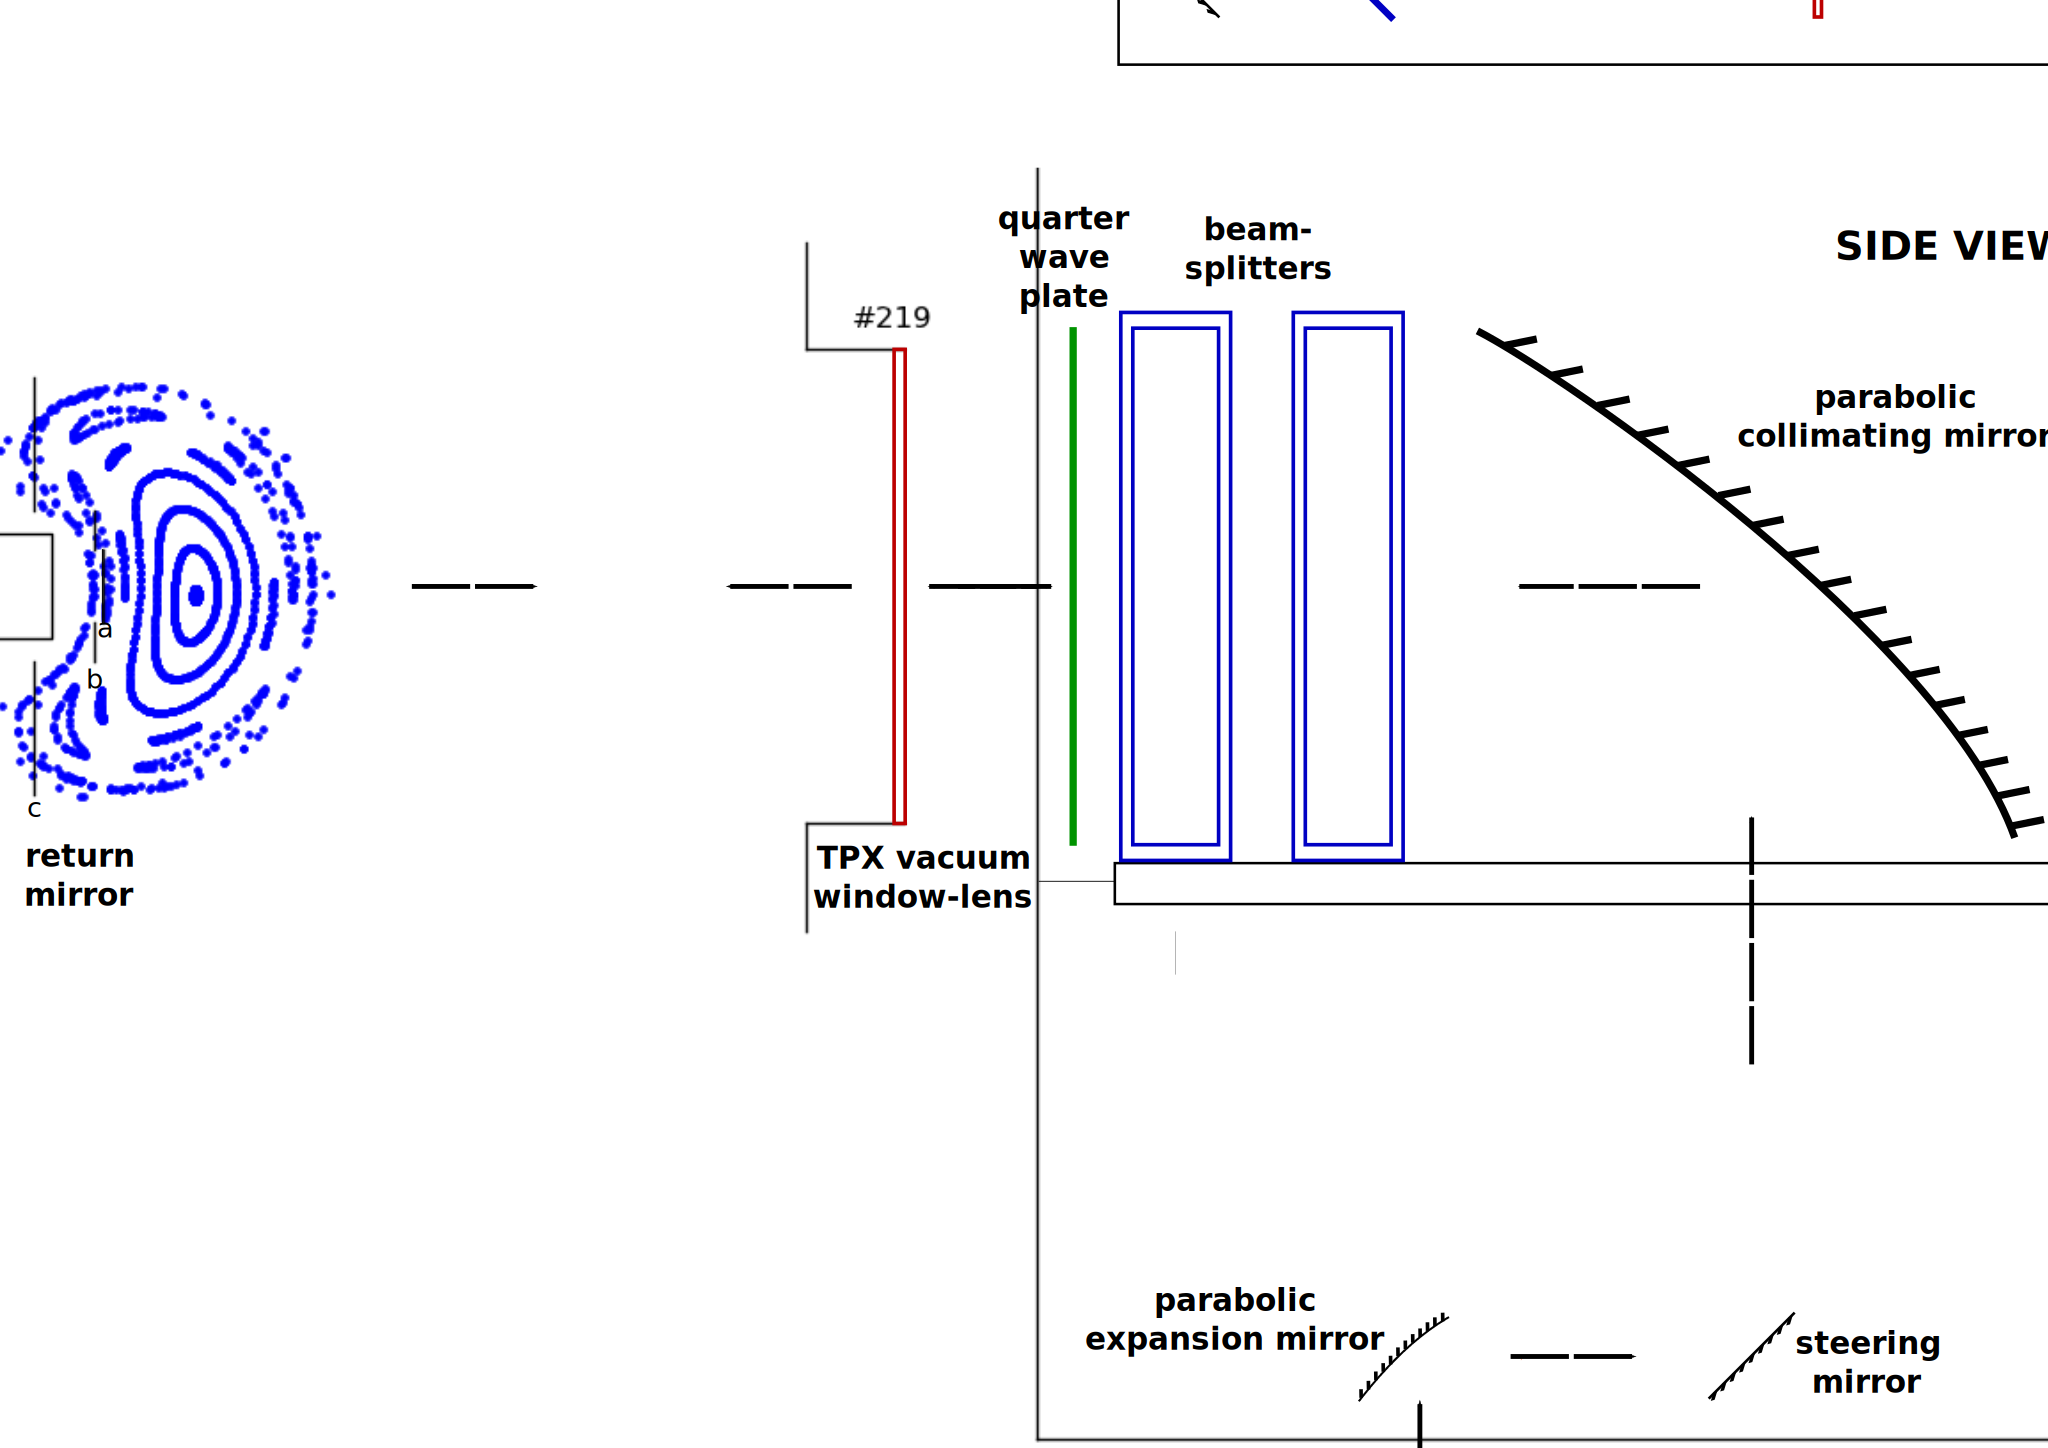
\includegraphics[width=\columnwidth]{figures/optical_component_layout_phaseii}
\caption{Overview of the optical layout.}
\label{fig:overview_schematic}
\end{figure}

\subsection{Gaussian beam modeling and FDTD simulations}
%FG & BDB
Beam dynamics may also be of value, possibly including FDTD simulations. Fresnel lens, quarter-wave plate, and imaging.
\thispagestyle{empty}
%Layout and components including mirrors, lens design, beamsplitter
%details and detector array.
%Beam dynamics may also be of value.
%Cover imaging arrangement, possibly including FDTD simulations.
\subsubsection{Beam modeling}


\subsubsection{FDTD simulations}

